% Created: 12-FEB-2021
% Revised: 
%
% VERSION 0.1
%
\documentclass{article}

\usepackage{graphicx} % screenshots
\usepackage{fancyhdr} % Required for custom headers
\usepackage{lastpage} % Required to determine the last page for the footer
\usepackage{extramarks} % Required for headers and footers
\usepackage{paralist} % compact lists
\usepackage{parskip} % more space between paragraphs
\usepackage{textcomp} % straight quotes for code
\usepackage{hyperref} % for hyperlinks in the document
\usepackage{tabularx} % for text-wrapping in tables
\usepackage{tikz} % diagrams
\usetikzlibrary{shapes.geometric, arrows, positioning}

\hypersetup{
    colorlinks=true
}

% Set up the header and footer
\pagestyle{fancy}
\lhead{\hmwkAuthorName} % Top left header
\chead{\hmwkTitle} % Top center head
\rhead{\hmwkClass} % Top right header
\lfoot{\lastxmark} % Bottom left footer
\cfoot{} % Bottom center footer
\rfoot{Page\ \thepage\ of\ \protect\pageref{LastPage}} % Bottom right footer
\renewcommand\headrulewidth{0.4pt} % Size of the header rule
%\renewcommand\footrulewidth{0.4pt} % Size of the footer rule

\setlength\parindent{0pt} % Removes all indentation from paragraphs

%----------------------------------------------------------------------------------------
%	DOCUMENT STRUCTURE COMMANDS
%	Skip this unless you know what you're doing
%----------------------------------------------------------------------------------------

% Header and footer for when a page split occurs within a problem environment
\newcommand{\enterProblemHeader}[1]{
% \nobreak\extramarks{#1}{#1 continued on next page\ldots}\nobreak
% \nobreak\extramarks{}{#1 continued on next page\ldots}\nobreak
}

% Header and footer for when a page split occurs between problem environments
\newcommand{\exitProblemHeader}[1]{
% \nobreak\extramarks{#1 (continued)}{#1 continued on next page\ldots}\nobreak
\nobreak\extramarks{#1}{}\nobreak
}

\setcounter{secnumdepth}{0} % Removes default section numbers
\newcounter{homeworkProblemCounter} % Creates a counter to keep track of the number of problems

\newcommand{\homeworkProblemName}{}
\newenvironment{homeworkProblem}[1][Problem \arabic{homeworkProblemCounter}]{ % Makes a new environment called homeworkProblem which takes 1 argument (custom name) but the default is "Problem #"
\stepcounter{homeworkProblemCounter} % Increase counter for number of problems
\renewcommand{\homeworkProblemName}{#1} % Assign \homeworkProblemName the name of the problem
\section{\homeworkProblemName} % Make a section in the document with the custom problem count
\enterProblemHeader{\homeworkProblemName} % Header and footer within the environment
}{
\exitProblemHeader{\homeworkProblemName} % Header and footer after the environment
}

\newcommand{\problemAnswer}[1]{ % Defines the problem answer command with the content as the only argument
\noindent\framebox[\columnwidth][c]{\begin{minipage}{0.98\columnwidth}#1\end{minipage}} % Makes the box around the problem answer and puts the content inside
}

\newcommand{\homeworkSectionName}{}
\newenvironment{homeworkSection}[1]{ % New environment for sections within homework problems, takes 1 argument - the name of the section
\renewcommand{\homeworkSectionName}{#1} % Assign \homeworkSectionName to the name of the section from the environment argument
\subsection{\homeworkSectionName} % Make a subsection with the custom name of the subsection
\enterProblemHeader{\homeworkProblemName\ [\homeworkSectionName]} % Header and footer within the environment
}{
\enterProblemHeader{\homeworkProblemName} % Header and footer after the environment
}

%----------------------------------------------------------------------------------------
%	NAME AND CLASS SECTION
%----------------------------------------------------------------------------------------

\newcommand{\hmwkTitle}{Welcome to K Division} % Assignment title
\newcommand{\hmwkDueDate}{March 8, 2021} % Due date
\newcommand{\hmwkClass}{CP490} % Course/class
\newcommand{\hmwkClassTime}{TBD} % Class/lecture time
\newcommand{\hmwkClassInstructor}{TBD} % Teacher/lecturer
\newcommand{\hmwkAuthorName}{Mr. Klein} % Your name

%----------------------------------------------------------------------------------------
%	TITLE PAGE
%----------------------------------------------------------------------------------------

\title{
\vspace{2in}
\textmd{\textbf{\hmwkClass:\ \hmwkTitle}}\\
\normalsize\vspace{0.1in}\hmwkDueDate\\
\vspace{0.1in}\large{\textit{\hmwkClassInstructor\ \hmwkClassTime}}
\vspace{3in}
}

\author{\textbf{\hmwkAuthorName}}
\date{} % Insert date here if you want it to appear below your name

\begin{document}

\maketitle\thispagestyle{empty}

%----------------------------------------------------------------------------------------
%	Course Parameters
%----------------------------------------------------------------------------------------
\begin{homeworkProblem}[Overview]

  You are going to be part of a fictional, global corporation that produces interactive cloud applications. You will be split into teams. Each team will own a specific part of the application and you will be responsible for designing, programming, and deploying it. You will need to interact with your peer teams to ensure that all parts of the application work together. You will also need to interact with the product owner to ensure that your deliverables meet requirements, and interact with a fictional operations team who will also stand up your application.

\begin{homeworkSection}{Course Format}
  The class will meet as a whole 3 times per week for an hour. During that meeting, time will be spent on:
	\begin{compactitem}
		\item (15 minutes) Team status (3 x 5 minutes)
		\item (30 minutes) Architecture / Design / Document Reviews, as needed
		\item (30 minutes) Problem solving or bootstrapping
	\end{compactitem}

	Team status is a summary of activities -- what your team worked on, and what's up next.
	
	Teams will need to present their solutions to the group for feedback and review. Teams should be prepared to discuss the technical details of the problems they are solving. Teams should be prepared with any diagrams and supporting reference material so that the class is able to understand and contribute feedback. Discussion is to be focussed on gaps and potential trouble areas.

	The time can also be used to help teams solve problems encountered, whether that's a technical issue or help in coordinating deliverables between teams.
	
	Lastly, this project is likely to use technology unfamiliar to the class. I will lead sessions to cover this material.
\end{homeworkSection}


\begin{homeworkSection}{Evaluation Criteria}
	This class is PASS / FAIL, so no graded marks are given. A PASS in this class is earned by demonstrating that you provided value to your team and helped achieve its goals. Failure would represent individuals that did not contribute technically, were unable to work within agreed-upon processes, and could not coordinate with other teams.
	
	You will write a summary of your individual contributions to the project to help with this, which I will combine with my own observations.
\end{homeworkSection}


\begin{homeworkSection}{General Expectations}
	I am going to hold you to the same standards that I have for junior development staff. That is, I know you're capable of doing the work, and you will need help learning the tools and processes.

	While I hope that the class as a whole produces a working application that everyone can take pride in, it's entirely possible that it won't come together as expected. That's ok -- my goal is that you work within software processes, talk with other teams, debate your ideas, and learn unfamiliar tools.

	To that end, we will operate according to these values:

	\begin{compactitem}
		\item \textbf{Respect always}: Assume that people are acting in good faith. Earn the trust of your teammates and give it, too.
		\item \textbf{Fundamentals first}: Value the basics of testing, designing, and communicating. Creating complex solutions is possible through the diligent, regular application of focussed effort. Know your tools and practice.
		\item \textbf{Start simple and iterate}: Value taking action above waiting for answers. Reach out instead of disengaging. Sharing a partial solution today is far more valuable than trying to have everything working next week.
	\end{compactitem}
\end{homeworkSection}

\end{homeworkProblem}


%----------------------------------------------------------------------------------------
%	Problem description
%----------------------------------------------------------------------------------------
\begin{homeworkProblem}[Project]

  K Division produces a platform for multiplayer online text-based roleplaying games\footnote{that is, MUDs: \url{https://en.wikipedia.org/wiki/MUD}} using their proprietary, leading--edge COAL Engine\footnote{\textbf{C}oncurrent \textbf{O}nline \textbf{A}dventure \textbf{L}and Engine}. Since they're a startup, the game engine isn't written yet, so some of you are going to need to do that. They don't have a front-end yet, either. Or a database backend. It's not much of a company, really, but the investors are thrilled!


\begin{homeworkSection}{Background}
	MUDs, and their single--player cousins, the Text Adventure, were precursors to Massively Multiplayer Online Roleplaying Games (MMORPGs). Players connect to a server using a command line terminal, read descriptions of the environment their characters are in, and type commands. Those commands allow the player to travel, engage in combat, manage inventory, craft, and interact with other players.
	
	If you haven't played one of these, then you might want to try \href{https://play.achaea.com/}{Achaea}, which is a rather more sophisticated version of what we're trying to create.

	Why text-based? If it's going to be a \textit{game}, why not have it be in Unity or Unreal? From a systems design standpoint, that would place emphasis in the wrong place. Rather, formulating the project this way provides a frame for a multi--tier application with a user interface, database, and API, along with integration with other software platforms. Insofar as this is a \textit{game}, it's a rather serious one.
\end{homeworkSection}

\begin{homeworkSection}{Playing the Game}
	In the game, a user takes on the role of a character that wanders around a virtual world, solving puzzles, battling monsters and other characters, amassing various items, and conversing with other users.
	
	The user is presented with a text description of their character's current location and a command line prompt. For example\footnote{This is from \textit{Zork I: The Great Underground Empire} (Infocom, 1980)},

	\begin{verbatim}
		West of House
		You are standing in an open field west
		of a white house, with a boarded front
		door.
		There is a small mailbox here.

		>
	\end{verbatim}

	You can see the various parts of text:
	\begin{compactitem}
		\item \textbf{title}: West of House
		\item \textbf{description}: You are standing in \dots
		\item \textbf{item list}: A small mailbox
		\item \textbf{prompt}: The `$>$' character
	\end{compactitem}

	Descriptions may also include lists of:

	\begin{compactitem}
		\item valid exits, insofar as the player character can see
		\item other player characters in the same place
		\item monsters (non--player characters)
	\end{compactitem}
	
	The user then types a command. For example, \texttt{GO EAST} or \texttt{OPEN MAILBOX}.
	
	The game processes the command and replies with a new description, and another prompt. That's it -- that is the core interface and gameplay. That is,

	\begin{compactitem}
		\item The game server presents a block of text
		\item User types in a command
		\item Game server processes text, updating the game state
		\item Repeat!
	\end{compactitem}
\end{homeworkSection}


\begin{homeworkSection}{Game Objects}
	There are five types of objects in the COAL engine:
	\begin{compactitem}
		\item \textbf{Rooms}: These are the locations inhabited by the player characters
		\item \textbf{Items}: Objects that the player character interact with, such as boxes, lanterns, weapons, etc.
		\item \textbf{Characters}: The internal representation of a user's character, capturing the game state
		\item \textbf{Monsters}: Non-player characters, hostile or benevolent
		\item \textbf{Actions}: These define how the game engine responds to user commands
	\end{compactitem}

\begin{table}
	\begin{tabularx}{\textwidth}{|r|X|}
		\hline
		Property & Description \\
		\hline \hline
		Title & Short name for a room, e.g. \texttt{West of House} \\
		Description & Longer text with details of what the room looks like \\
		Exits & A list of visible directions mapped to destinations, e.g. \texttt{East $\rightarrow$ House} \\
		\hline
	\end{tabularx}
	\caption{Room properties}
	\label{tab:room-properties}
\end{table}

\begin{table}
	\begin{tabularx}{\textwidth}{|r|X|}
		\hline
		Property & Description \\
		\hline \hline
		Name & Short name for the item, e.g. \texttt{Sting} \\
		Aliases & Other words that can be used for the item, e.g. \texttt{sword} \\
		Description & Additional details, e.g. \texttt{An Elvish short-sword that is somewhat fond of spiders} \\
		Attack value & Value of base damage dealt in combat \\
		Defense value & Amount of damage absorbed in combat \\
		Location & Current room the object is in (or none, if it's inside something else or in a player's inventory) \\
		\hline
	\end{tabularx}
	\caption{Item properties}
	\label{tab:item-properties}
\end{table}

\begin{table}
	\begin{tabularx}{\textwidth}{|r|X|}
		\hline
		Property & Description \\
		\hline \hline
		Name & In--game name of the player character \\
		Location & Room where the character is located \\
		Health & Amount of damage that can be sustained \\
		Inventory & Items acquired by the player character \\
		Flags & A list of key--value pairs for keeping game state (e.g. \texttt{HAS-SEEN-WELCOME-TEXT} $\rightarrow$ \texttt{TRUE}) \\
		User & User account the player character belongs to \\
		\hline
	\end{tabularx}
	\caption{Character properties}
	\label{tab:character-properties}
\end{table}

\begin{table}
	\begin{tabularx}{\textwidth}{|r|X|}
		\hline
		Property & Description \\
		\hline \hline
		Name & Short name for the monster \\
		Location & Room where the monster is located \\
		Health & Amount of damage that can be sustained \\
		Inventory & Loot carried by the monster \\
		\hline
	\end{tabularx}
	\caption{Monster properties}
	\label{tab:monster-properties}
\end{table}

\begin{table}
	\begin{tabularx}{\textwidth}{|r|X|}
		\hline
		Property & Description \\
		\hline \hline
		Command & A list of static text and arguments describing the syntax of the action, e.g. \texttt{GO !DIRECTION!} \\
		Events & A list of \textit{(condition, true-response, error message)} tuples, where all the conditions of given event must be true for the true-response to execute. The responses are lists of game engine functions to manipulate any mutable game state \\
		\hline
	\end{tabularx}
	\caption{Action properties}
	\label{tab:action-properties}
\end{table}

	Each of the object types has a number of \textit{properties}. Those properties are either \textit{mutable}, meaning that they can be changed as part of playing the game, or \textit{immutable}. Properties that are immutable can only be edited by game authors outside of the game and cannot be changed through player interactions directly.

	The locations in the game are collectively referred to as ``rooms,'' even though they could be describing outdoor locations, caves, spaceships, or more abstract settings\footnote{For example, \href{https://en.wikipedia.org/wiki/A_Mind_Forever_Voyaging}{A Mind Forever Voyaging} (Infocom, 1985)}. A list of properties is given in Table \ref{tab:room-properties}. If a user is entering the location for the first time, then the full description is shown. Otherwise, only the short title is shown. A list of directions, like \texttt{NORTH} or \texttt{UP} are mapped against other rooms to connect them. This list of exits is usable by, and shown to, the player. The title, description, and exits are all immutable properties.

	Items are what users manipulate in the game: weapons, armour, keys, treasure, and so on. The properties of items are given in Table \ref{tab:item-properties}. An item has a name, but also possibly aliases. For example, there may be a book with the name \textit{Hitchhiker's Guide} that also has an alias of \textit{book} and \textit{guide}, so the user can type: \texttt{GET HITCHHIKER'S GUIDE} or \texttt{GET GUIDE} or \texttt{GET BOOK} interchangeably. Attack and defense values pertain to combat, and while usually associated with weapons and armour, could just as easily have non--zero values for kitchen utensils or ukuleles. It's easier to assign everything values (even if zero) then to introduce different types of items. Last, the only mutable property is the item location, since items (in general) can be added to a player character or monster inventory.

	Table \ref{tab:character-properties} lists the properties of player characters. These are the proxies for users, and so all the state in this object is mutable. For the sake of combat, the player character has health, an integer value, that can be changed by combat damage, items, and events. Flags allow the game engine to track other kinds of game state. For example, the player character may be poisoned, or using a potion that lasts for a given number of moves. This key--value mechanism provides an open--ended way to create and manage character data. Each player character is associated with one and only one user account, but a user account may have multiple player characters.

	Monsters barely differ from player characters, except that they are not controlled by users directly; see Table \ref{tab:monster-properties}. Further, the name of a monster is immutable, but all the remaining fields are game state (mutable).

	Last, the properties of actions are given in Table \ref{tab:action-properties}. The functionality of the game is described using actions. All the properties are immutable. The game engine considers each action command as a pattern -- it will try to match the user input against a single action. The list of events for that command are then evaluated. An event consists of a set of conditions (e.g. is the player in a certain room?). If the conditions are met, then the true-response is evaluated. Otherwise, an error message is added to the response back to the user. All events for a given action are evaluated -- the game engine doesn't stop on the first failure or success.
\end{homeworkSection}

\begin{homeworkSection}{Creating Game Content}
	Game play requires game content. Classically, in MUDs, once you attained a certain rank within the game\footnote{sometimes called wizard status}, you were allowed to author game content. For some early or small MUDs, this meant recompiling the source code. The prevailing idea, however, was that you could add new content as metacommands in the game.

	For this project, game content creation should be separate from gameplay, but it is an integral part of the platform and users should be able to create rooms, items, and monsters. 
\end{homeworkSection}

\begin{homeworkSection}{Design and Architecture Principles}
  Cloud computing is a popular way of deploying large-scale enterprise business applications. Companies large and small outsource their infrastructure and host their applications with cloud computing companies -- be it Amazon, Microsoft, Google, or others. One reason for Amazon's success as a cloud provider is their emphasis on creating \textit{platforms}. The same website that let them sell books became the same one that lets everyone else sell, well, everything. It's a \textit{platform} for online sales. Further, Amazon Web Services (AWS) is consumed by Amazon internally, meaning that the services Amazon sells are the same ones it uses to run their business.
  
  Similarly, the K Division application is a \textit{platform} for MUDs. The game that we should be able to play at the end of this is a \textit{demonstration of the platform} more than a shrink--wrap product\footnote{read more about this here: \url{https://gist.github.com/chitchcock/1281611}}.
  
  The way we build platforms is through \textit{Application Programming Interfaces} (APIs). APIs are everywhere. Google has \href{https://developers.google.com/apis-explorer}{all kinds}. Zoom? They \href{https://marketplace.zoom.us/docs/api-reference/zoom-api}{have an API}. Do you use Slack? They \href{https://api.slack.com/}{have an API} to write bots. So \href{https://developers.facebook.com/}{does Facebook}. Maybe you play games and use Discord. Here's \href{https://discord.com/developers/docs/intro}{their API}.
  
	An \textit{API} is a kind of programming contract. If I provide your service with input that conforms to your specification, then your service agrees to return a result in a given format. For example, an API can be written to accepts and return JavaScript Object Notation (JSON)\footnote{see \href{https://en.wikipedia.org/wiki/JSON}{Wikipedia}} objects. To describe APIs, we are going to use \href{https://swagger.io/specification/}{OpenAPI documents}. OpenAPI is a way of writing descriptions of API contracts in a way that lets us use other code generation software tools to create clients and servers for us.

  You will be given an OpenAPI document that specifies the public--facing API of the COAL Engine. You will negotiate internal APIs with your peer teams. I expect to be able to write my own game client against this public API and use it to explore your work. You may need to negotiate changes to the public API, if it doesn't let you fulfill your requirements.
\end{homeworkSection}

\begin{homeworkSection}{Application Architecture}
	
\begin{figure}
\centering
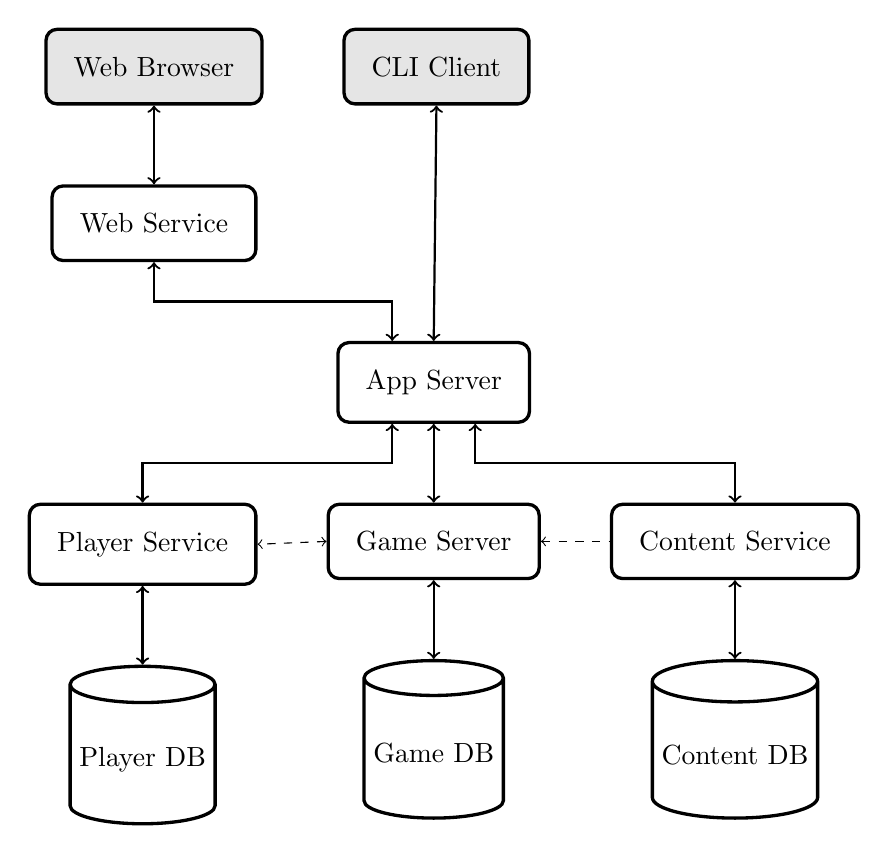
\begin{tikzpicture}
	\tikzset{
    mynode/.style={rectangle,rounded corners, draw=black, very thick, inner sep=1em, text centered},
		usernode/.style={rectangle,rounded corners, draw=black, very thick, inner sep=1em, text centered, fill=black!10},
		dbnode/.style={cylinder,shape border rotate=90,draw=black, very thick, minimum height=2cm, aspect=0.25},
	}
	\node[mynode] (api) at (0,0) {App Server};
	\node[mynode, above left = of api] (webserver) {Web Service};
	\node[usernode, above = of webserver] (webui) {Web Browser};
	\node[usernode, right = of webui] (cli) {CLI Client};

	\draw[<->, thick] (webui.south) -- (webserver.north);

	\draw[<->, thick] (cli.south) --  (api.north);
	\draw[<->, thick] (webserver.south) -- ++(0, -0.5) -| (api.135);

	\node[mynode, below left = of api] (ps) {Player Service};
	\node[mynode, below = of api] (gs) {Game Server};
	\node[mynode, below right = of api] (cs) {Content Service};

	\draw[<->, thick] (api.225) -- ++(0, -0.5) -| (ps.north);
	\draw[<->, thick] (api.south) -- (gs.north);
	\draw[<->, thick] (api.315) -- ++(0, -0.5) -| (cs.north);

	\draw[<->, dashed] (gs.west) -- (ps.east);
	\draw[<-, dashed] (gs.east) -- (cs.west);

	\node[dbnode, below = of gs] (gdb) {Game DB};
	\node[dbnode, below = of ps] (pdb) {Player DB};
	\node[dbnode, below = of cs] (cdb) {Content DB};

	\draw[<->, thick] (gs.south) -- (gdb.north);
	\draw[<->, thick] (ps.south) -- (pdb.north);
	\draw[<->, thick] (cs.south) -- (cdb.north);
\end{tikzpicture}
\caption{Overall Application Architecture}
\label{fig:arch}
\end{figure}

The overall application architecture is given in Figure \ref{fig:arch}. There are three tiers:
\begin{compactitem}
	\item \textbf{User Interface}: The class is responsible for the web server front--end where users can play the game, manage their account, and so forth.
	\item \textbf{Application Tier}: The application server coordinates activity between the data tier and the UI tiers. It exposes the public API, makes corresponding requests to the data tier servers, and formats the responses back to the UI tier clients.
	\item \textbf{Data Tier}: The player, game, and content servers manage their respect portions of the COAL engine. Since each of these services can be expanded in different ways, they each have their own database components. The game service communicates with the player service to update state, as well as the content service to fetch data. 
\end{compactitem}

The App Server has no direct access to the databases, and does not know the schema for the data. A database is a shared resource, and having a service in front of it can protect it from being overwhelmed. This is also a pattern for providing horizontal scaling. That is, the App Server process can be duplicated until there are enough instances to handle the load from users independently of the back--end resources. The databases can be scaled vertically -- that is, more resources given to the database instance so that it can store the data and process requests efficiently.

\end{homeworkSection}


\begin{homeworkSection}{Web Service}
	The web service provides the front--end for the game. Users must be able to manage their account and game characters. They must also be able to play the game itself using an interactive console.
\end{homeworkSection}


\end{homeworkProblem}


\end{document}